\documentclass[../main.tex]{subfiles}

\begin{document}

\chapter{Methodology} \label{chapter:methodology}

This chapter highlights the specific algorithms and datasets used as well as the setup for each performed experiment.

\section{Data} 

In order to answer some of the specified research questions, a total of nine labelled datasets were obtained. Six of these were obtained from previous research \cite{kamei2013large} and the other three were collected using software projects at King.

\subsection{Data From Previous Research}

In their work \textit{A Large-Scale Empirical Study of Just-in-Time Quality Assurance}, Kamei et al. provided 6 labelled datasets \footnote{The six previous datasets can be found here http://research.cs.queensu.ca/~kamei/jittse/jit.zip} which contained commit metadata from open source projects \cite{kamei2013large}. These six datasets correspond to the first six rows of Table \ref{table:allData}. 
\vspace{10pt}

\begin{table}[h]
    \centering
    \caption{\textbf{All datasets used in experiments}}
    \begin{tabular}{|c c c c c|} 
    \hline
    \textbf{Project} & \textbf{Time} & \textbf{\# Commits} & \textbf{\% Buggy} & \textbf{Approximate SZZ}\\ 
    \hline\hline
     Bugzilla & 08/1998-12/2006 & 4,260 & 36\% & No\\ 
     \hline
    Columba & 11/2002-07/2006 & 4,455 & 31\% & Yes\\
    \hline
    JDT & 05/2001-12/2007 & 35,386 & 14\% & No\\
    \hline
    Platform & 05/2001-12/2007 & 64,250 & 14\% & No\\
    \hline
    Mozilla & 01/2000-12/2006 & 98,275 & 5\% & No\\
    \hline
    PostgreSQL & 07/1996-05/2010 & 20,431 & 25\% & Yes\\
    \hline
    C1 &  - & 32,661 & - & Yes\\ %31.6\%
    \hline
    C2 &  - & 121,636 & - & Yes\\ %33\% 
    \hline
    C3 &  - & 57,802 & - &Yes\\ %30\% 
    \hline
    Total & - & 439,156 & - & - \\ %30\% 
    \hline
    \end{tabular}
    \label{table:allData}
\end{table}

\subsection{Newly Collected Data}

As seen in chapter \ref{chapter:technical_contribution} of the report, the implemented data collection tool was used to collect data on several proprietary projects at Kings. The data that was collected included all commits from these project except those that represented merges between branches in Git. Merge commits were excluded because they represent a collection of several commits as one large change, hence distorting the dataset as an outlier. Also, merge commits are created automatically by Git rather than a developer and defect prediction tools intend to predict on commits made by developers. The names and percent of buggy commits for the commercial projects in table \ref{table:allData} are anonymous for confidentiality reasons. Most of the features in the new datasets were computed in an identical manner to those in the Kamei datasets. The reason for not including the exact same set of features as the old datasets was due to limitations in time when implementing the tool. 

\subsection{Features Used}

Table \ref{table:Features} describes the individual features used in all provided datasets. These features can be directly extracted using Git commands such a \texttt{git log}. The column \textbf{Datasets used in} in Table \ref{table:Features} indicates if a feature is included in the old datasets, new datasets or in both. The features FIX, DAY and HOUR are categorical features which can only take a finite number of values whereas the remaining features are all integers or real valued. 

\subsection{Data Preprocessing}

First, the features with a high positive Pearson correlation coefficient were removed in order to simplify the model. Next, due to the fact that features associated with commits are not normally distributed, log transforms were applied to all continuous valued features using the function $f(x) = ln(x+1)$. This function was used because some features could take a value of 0 and the standard log function would make these values undefined. The data was then standardized which ensured that the mean and standard deviation of each features was 0 and 1 respectively. To deal with multilabel categorical features such as "DAY", these feature were represented using a one-hot encoding. In order to deal with the class imbalance, random undersampling is performed on the training set in order to produce a dataset with an equal number of \textit{risky} and \textit{not risky} commits. The steps undertaken in this stage were similar to what Kamei et al. performed \cite{kamei2013large} in order to ensure results would be comparable under similar conditions. 

\begin{table}[H]
    \centering
     \caption{\textbf{Features used in Table \ref{table:allData} datasets}}
   \begin{tabular}{|p{15mm} |p{85mm} |p{30mm} |} 
        \hline
        \textbf{Name} & \textbf{Description} & \textbf{Datasets used in}\\ 
        \hline\hline
        NS & Number of modified subsystems & Both\\
        \hline
        ND & Number of modified directories & Both\\
        \hline
        NF & Number of modified files & Both\\
        \hline
        Entropy & Distribution of modified code across each file & Both\\
        \hline
        LA & Lines of code added& Both\\
        \hline
        LD & Lines of code deleted & Both\\
        \hline
        LT & Lines of code in a file before the change & Old \\
        \hline
        FIX & Whether or not the change is a defect fix & Both\\
        \hline
        NDEV & The number of developers that changed the modified files & Old \\
        \hline
        AGE & The average time interval between the last and the current change & Old\\
        \hline
        NUC & The number of unique changes to the modified files & Old\\
        \hline
        EXP & Developer experience & Old \\
        \hline
        REXP & Recent developer experience & Old \\
        \hline
        SEXP & Developer experience on a subsystem & Old \\
        \hline
        DAY & The day of the week & New\\
        \hline
        HOUR & An integer between 0 and 23 & New\\
        \hline
        WORDS & The number of words in a commit message & New\\
        \hline

\end{tabular}
    \label{table:Features}
\end{table}

\section{Experimental Setup}

All scripts for the experiments were implemented in Python 3. The Scikit-learn library was used to create, train and evaluate machine learning models such as logistic regression, random forest, Adaboost and K-nearest neighbours. The XGBoost model was provided under a separate python package \footnote{XGBoost documentation https://xgboost.readthedocs.io/en/latest/}. The Pandas library was used for preprocessing the datasets and MatplotLib was used for all graphs and visualisations. An open-source implementation of the self-training algorithm was used in experiments for the first research question \footnote{https://github.com/tmadl/semisup-learn/blob/master/frameworks/SelfLearning.py}. When generating random floating point numbers, the random library was used with a seed of 42. All of the scripts were executed on hardware provided at King. All scripts were executed on high-end build servers provided at King. 

\section{Experiments}

This section describes the exact methods used to answer the four research questions mentioned in the introduction. 

\subsection{Experiments for RQ1}

For this question, the performance of five classifiers was evaluated using 10-fold cross validation. The datasets used in the evaluation are the six open source projects from table \ref{table:allData}. Due to limitations in time, it was not possible to reimplement models from previous research and apply them on the new datasets. 

\subsubsection{Classification Models Used}

The chosen models were logistic regression (LR), random forest (RF), AdaBoost (ADA), XGBoost (XGB) and K-nearest neighbours (KNN). Logistic regression was chosen in order to observe how self-training affects a linear classification model. Random forest was chosen as tree based methods tend to outperform linear models for software defect predictions. AdaBoost and XGBoost were chosen to compare boosting methods with bagging methods such as random forest. Finally, K-nearest neighbours was selected to have another non parametric model that was not tree based. No approaches based on artificial neural networks were used 
because they require a lot of data to perform well. When creating defect prediction models for smaller projects, neural networks may not be as viable. Also, when evaluating the usefulness of the self-training algorithm, the performance of neural networks may be much lower than in normal circumstances as they would have access to less data.

\subsubsection{Parameters for Classification Models}

The parameters for logistic regression was the \textit{lbfgs} solver and 5000 maximum iterations. Random forest used 100 estimators and K-nearest neighbours used $k=5$ for the number of neighbours. All other parameters for these models used the default values provided by the scikit-learn package in Python. All classifiers had their classification threshold set to 0.5. As binary classifiers output a probability between 0 and 1, a threshold of 0.5 indicates that any value above 0.5 becomes classified as risky and any value below it is labelled as not risky. 

\subsubsection{Performance Metrics Used}

When evaluated on the test set, the performance metrics that were measured were precision, recall and F1-score. As a baseline, all models are compared to a random model which outputs each possible label with equal probability. 

\subsection{Experiments for RQ2}

In order to answer this question, the performance of various classifiers must be compared when they are trained in a supervised manner as opposed to a when using self training algorithm (see \ref{section:selfTrain}). The specified null hypothesis for this experiment would be:

\begin{center}
   \textit{$H_0:$ "The self-training algorithm does not lead to a change in performance compared with the base performance of five specified supervised algorithms when applied to Just-In-Time defect predictions."}
\end{center}


\subsubsection{Evaluating Self-Training Using Cross Validation}

The evaluation procedure involves providing supervised models and their self-trained counterpart with training data and evaluating their performance on test data. Every commit in each dataset is labelled so in order to simulate a setting where a model has access to labelled and unlabelled data, a portion of labels must be removed. Although the supervised classifier will only be able to train on the labelled instances, the semi-supervised classifier can make use of labelled and unlabelled instances. Both classifiers are ensured to train on the exact same set of labelled training data. 

\begin{figure}[H]
    \centering
    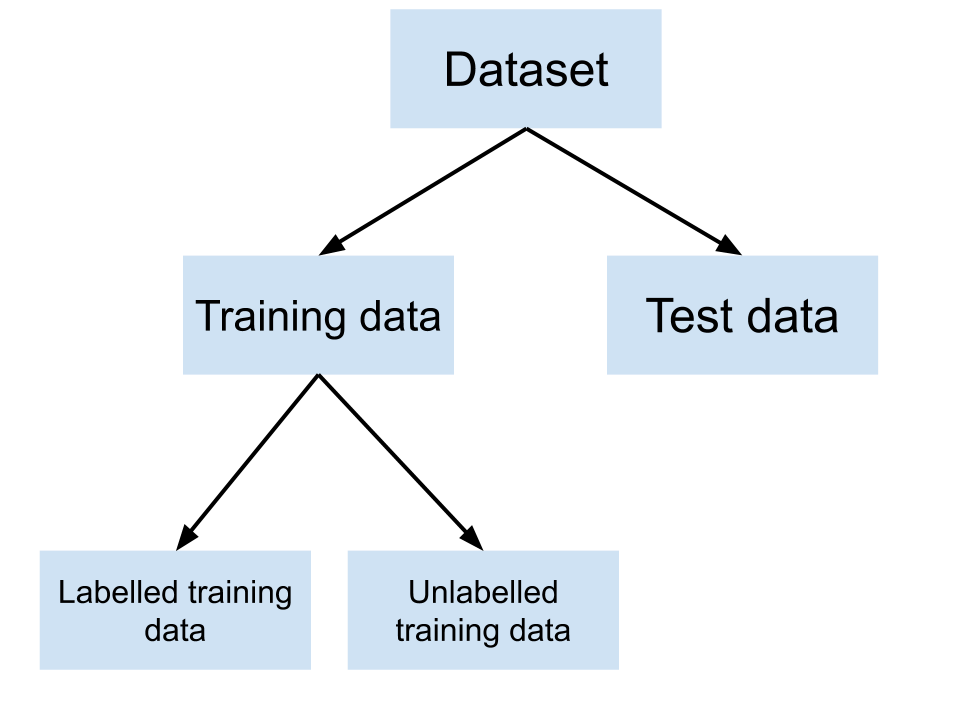
\includegraphics[scale=0.4]{images/Methodology/data_split.png}
    \caption{The supervised model trains exclusively on the \textbf{labelled training data} whereas the self-trained model uses both \textbf{labelled training data} and \textbf{unlabelled training data}}
    \label{fig:train_test_labelled_split}
\end{figure}


Algorithm \ref{algorithm:evaluation} is used repeatedly when measuring performance in each of the experiments. The models used in the experiments for this research question are identical to those used for research question 1. In the algorithm below, $D$ is a dataset, $M \in \{LR, RF, ADA, XGB, KNN\}$ is the model type, $I$ is the maximum number of iterations the self-training algorithm runs for, $C$ is the confidence threshold for the self-training algorithm and $U$ is the fraction of training data that will be made unlabelled. In order to verify the specified null hypothesis above, three experiments were performed. 

\begin{comment}

Given our unprocessed datasets $\{D_1, D_2, ..., D_n\}$, a classifier $f$ can be evaluated on each dataset using $k$-fold cross validation where $k=10$, similar to previous research. Given the parameters $I, C, U$ such that:
\end{comment}
\begin{comment}
\begin{enumerate}
         \item $D_{train}^L$ only has labelled instances ($|D_{train}^L|=(1-U) \cdot |D_{train}|$)
         \item $D_{train}^U$ only has unlabelled instances ($|D_{train}^U|=U \cdot |D_{train}|$)
\end{enumerate} 
\begin{description}
\item [$I$] is the max number of iterations for the self-training algorithm, $I=$\selfTrainMaxIter
\item [$C$] is the minimum confidence for a prediction on unlabelled data, $C \in \{0.8,0.85,0.9\}$
\item [$U$] is the fraction of instances that will have their labels removed,
$U \in \{0,0.1,0.2,0.3,0.4,0.5,0.6,0.7,0.8\}$ (U=0 indicates that all training data is untouched).  
\end{description}
\end{comment}

\begin{algorithm}
\caption{Evaluates the performance of semi-supervised vs supervised classifiers}
\label{algorithm:evaluation}
\begin{algorithmic}[1]
\Procedure{Evaluation(D, M, I, C, U)}{}
    \State MetricSet = \{Accuracy, Precision, Recall, F1-score\}
    \State Preprocess dataset $D$
    \State Randomly shuffle and partition the dataset $D$ into $k$ partitions
    \For{$i=1 \dots k$}
        \State $D_{test} :=$ the $i^{th}$ partition of $D$.
        \State $D_{train} :=$ the union of all other partitions
        \State Instantiate untrained models $f,f'$ of type $M$
        \State Train $f$ on $D_{train}$ using supervised learning
        \State Partition $D_{train}$ into $D_{train}^L, D_{train}^U$
        \State $X_L, y_L$ is obtained from $D_{train}^L$  
        \State $X_U$ is obtained from $D_{train}^U$
        \State Run \texttt{Self-Train($X_L, y_L, X_U, I, C, f'$)} to train $f'$ (see algorithm \ref{algorithm:selfTrain})
        \State Evaluate $f, f'$ on $D_{test}$ and record various performance metrics
        \State Discard the models $f, f'$
    \EndFor
    
    \For{metric in MetricSet}
        \State Compute mean, standard deviation of metric
    \EndFor
\EndProcedure
\end{algorithmic}
\end{algorithm}

To fully investigate how self-training affects classification models, a broad comparison of various models as well as a more in-depth analysis performed using the following experiemnts. 

\subsubsection{Evaluation for several models}

This experiment involves running algorithm \ref{algorithm:evaluation} for each of the five classification models and for each of the nine datasets. The number of iterations for self-training was set to 20, the percentage of labelled data was 20\% and the confidence threshold for the self-training algorithm was 0.8.  

\subsubsection{Varying the percentage of labelled data}

Here, algorithm \ref{algorithm:evaluation} ran on the C1 dataset using a random forest model with 100 estimators. The percentage of labelled data was varied from 10\% to 100\% with a step size of 10\%. The confidence thresholds used where 0.80, 0.85 and 0.90 and the number of max iterations for self-training was set to 20. The purpose of this experiment was to see after what point does the additional unlabelled data become useful and to see the trade-off between performance and the reduction in labelled data.

\subsubsection{Varying the number of iterations for self-training}

For this experiment, algorithm \ref{algorithm:evaluation} ran on the C1 dataset. The percentage of labelled data was set to 20\% and the confidence threshold at 0.9. The number of max iterations was varied from 5 to 100 with a step size of 5. This experiment was of interest because the self-training algorithm may possibly converge and the time spent using the algorithm can be reduced if its limits are known. 

\subsection{Experiments for RQ3}\label{section:case_study}

In order to evaluate this question, a case study was set up in order to evaluate the usefulness of these models on developers at King. Below is the proposed methodology for answering such a question objectively. One could define the null hypothesis as
\begin{center}
    \textit{$H_0:$ "An online machine learning tool that has trained on data that was labelled using ASZZ does not have an increased ability at spotting risky commits"}.
\end{center}

Seven developers which were working on the C3 project (see table \ref{table:allData}) were recruited and all of their latest commits on this project were recorded. The tool described in chapter 3 sent out predictions periodically to each participants so that they would only see predictions for commits that they authored and committed. Each participant was then asked to state if they agreed or disagreed with the prediction. In order to compare the model to a baseline, a random model was used to make predictions on the exact same set of commits that the trained model predicted on. The metrics that were recorded for both the trained and random model were accuracy precision and recall. As the commits produced by developers all happened to have a label of \textit{not risky}, manual labelling and the SZZ algorithm were used in order to find risky commits for the trained model to predict on. 

The theoretical values for each of these metrics can be derived for the random model. Given $n$ commits where $r$ have a true label of \textit{risky} and $p$ being the probability that the random model outputs the label \textit{risky}, the random model would then have the following metrics:

\begin{equation}
     TP = p \cdot r
\end{equation}

\begin{equation}
     TN = (1-p) \cdot (n-r)
\end{equation}

\begin{equation}
     FP = p \cdot (n-r)
\end{equation}

\begin{equation}
     FN = (1-p) \cdot r
\end{equation}

\vspace{10pt}

Using the quantities defined above, the accuracy, precision, recall and F1-score for the random model can be determined.
   
\begin{equation}\label{eqn:randAccuracy}
     Accuracy = \frac{pr+(1-p)(n-r)}{pr+p(n-r)+(1-p)(n-r)+(1-p)r} = (1-p) + \frac{r}{n}(2p-1)
\end{equation}

\begin{equation}\label{eqn:randPrecision}
    Precision = \frac{pr}{pr+p(n-r)} = \frac{r}{n}
\end{equation}

\begin{equation}\label{eqn:randRecall}
    Recall = \frac{pr}{pr+(1-p)r}=\frac{pr}{r} = p
\end{equation}


\begin{equation}\label{eqn:randF1}
    F1 = 2 \cdot \frac{Precision \cdot Recall}{Precision + Recall} = 2 \cdot \frac{pr}{pn+r} 
\end{equation}

\vspace{20pt}

Since our random model produced an equal probability for either label (p=0.5), it had an accuracy, precision, recall and F1-score of 0.5, $\frac{r}{n}$, 0.5 and $\frac{2r}{n+2r}$ respectively. The value of $\frac{r}{n}$ is the ratio of buggy commits to total commits and depends upon the dataset. If a trained model has learned what a defective commit is properly, it should be able to have a significant improvement over these values. 

\subsection{Experiments for RQ4}

In order to answer this question, qualitative interviews were performed at King which asked engineers from various backgrounds the following questions:

\begin{enumerate}
    \item Once you realize something is faulty with your software, how do you go about locating the origin of the bug ?
    \item What existing tools do you use that help you mitigate the risk of introducing bugs or to help detect bugs?
    \item What differences do you notice between faulty code and clean code ?
    \item What do you believe are the top causes of bugs ? 
\end{enumerate}

The motivation for asking these questions is that it may give an insight as to how software developers can identify code that contains defects. It could potentially also lead to new ideas for features that machine learning models could rely on. Additionally, it can help to build a solution that can benefit the developers in practice. 
\end{document}

